\documentclass{article}
\usepackage[utf8]{inputenc}
\usepackage{fullpage}
\usepackage{graphics}
\usepackage{txfonts}
\usepackage{url}
\setlength{\parindent}{0cm}
\begin{document}

\begin{center}\huge{Compétition le 15, 16 et 17 avril 2016\\à Bastogne}\end{center}
\vspace{3cm}

Ce weekend, nous avons prévu une compétition pour le groupe pré-compet (Miguel) et compet (Laurent).
Il s'agit du Mémorial Aernouts à Bastogne, un meeting compétitif avec finales:

\begin{itemize}
\item \textbf{Départ:} gare du midi, hall principal à 16h40 vendredi 15 avril 2016.\\\textbf{Ne soyez pas en retard, le train partira sans vous!}.
\item \textbf{Retour}: prévu dimanche le 17 avril vers 20h, gare du midi.
\item \textbf{Prix}: 60 euros tout compris: transports, logement, nouriture et inscriptions.
\item \textbf{Piscine}: Frédérik Deburghgraeve, rue Gustave Delperdange, 6600 Bastogne, Belgique\\\url{http://www.centresportifbastogne.be/}.
\item \textbf{Gîte}: rue Horritine, Michamp, 6600 Bastogne.
\item \textbf{Contact}: Laurent 0472 816 228, Miguel 0479 313 994
\end{itemize}

\paragraph{A prendre:}
Le gîte n'étant pas bien déservi par la TEC certains transports se feront à vélo.
Nous vous conseillons donc de voyager léger et en \textbf{sac-à-dos} (vous n'allez pas partir 6 mois en Martinique, sorry).
Aussi, toutes les collations et boissons sont comprises dans le prix et seront achetées sur place.

\begin{enumerate}
\item \textbf{Vélo}
\item \textbf{Draps de lits ou sac de couchage}
\item Maillot de bain
\item Lunette de natation
\item Bonnet du club
\item Un ou deux essuies
\end{enumerate}

\newpage

\begin{flushright}
\scalebox{0.65}{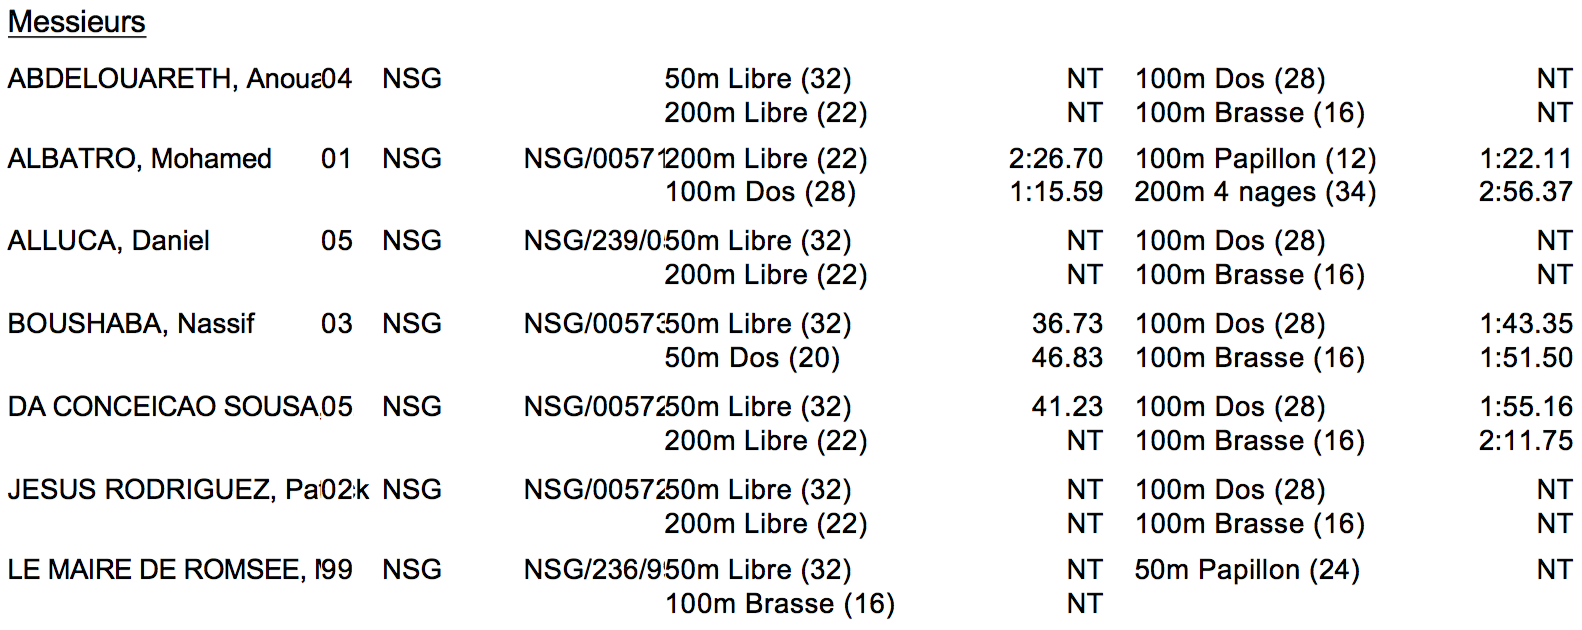
\includegraphics{1}}
\\
\scalebox{0.65}{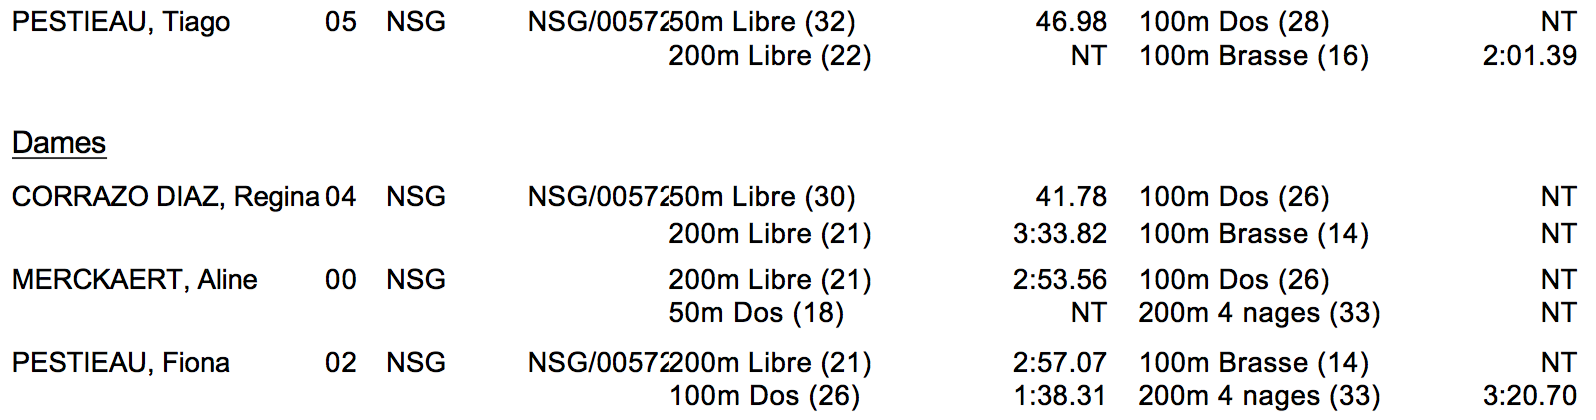
\includegraphics{2}}
\end{flushright}

\end{document}